\chapter{Data and Methods}
\label{sec:methods}
The purpose of this project was to evaluate the parameter thresholds for
tracking TCs in ICON simulation data. In the following section the settings
used for generating the simulation data and the algorithm itself will be
explained.
\section{Simulation Data}
\label{sec:data}
\subsection*{ICON Model}
The Icosahedral Nonhydrostatic Model (ICON) is developed by the German Weather
Service (DWD), the Max Planck Institute for Meteorology and several partner
institutes. As the name implies the grid is in a first step generated by
mapping the earths surface to an Icosahedron (platonic solid with 20
equilateral triangles as faces). The faces are then split up into smaller
triangles in order to achieve the desired resolution. The model then delivers
all typical meteorological quantities on this grid.
The model uses the fully compressible and non-hydrostatic version of the Euler
equations for the fundamental transport processes. Physical processes which
cannot be resolved with the grid size are then parametrised by using complex
functions that take into account the grid box mean values of the model
variables. Physical processes which need to be treated in this way include
solar and thermal radiation, cloud microphysics and turbulent transfer above
the earth's surface.\cite{dwd-icon}

\subsection*{Analysed simulation output}
The North Atlantic basin with its surrounding area ( TODO xx1 - xx2 lon and yy1
- yy2 lat) % TODO find out exact domain 
was simulated from the beginning of May until the beginning of December. The
output data is saved for every six hours.
Two different kinds of time lagged ensembles were used. Both used ERA5
reanalysis data for the initial weather state and the monthly boundary
conditions. The first however, labeled "ref", used the first day of each month
at 6:00 a.m. (TODO !confirm with Bernhard ) % TODO confirm time lagged ensemble with bernhard
as the monthly boundary conditions. The second ensemble, labeld "rm", used
monthly rolling mean boundary conditions based on the same reanalysis data.
The members within each of these two ensembles were created by varying the
initial weather state of the simulation. Namely each of the first 10 days of
May were used as initial conditions for a separate simulation run.
The output data from each run is mapped from the icosahedral to a
Latitude-Longitude grid in order to facilitate distance calculations.
Finally this results in 20 separate simulation runs that can be searched for
TCs.
%TODO RENAME STEPS TO TRACKING AND STITCHING AND THEN EXPLAIN
%TODO mention the amazing job I did in regards to vectorization
\section{Algorithm}
An existing algorithm developed by Bernhard Enz and inspired by \cite{orig-tracking} was improved in regards to runtime, robustness and
readability. The gained speed was used in order to run the algorithm on the
same simulation data but with different threshold values that decide wether a
TC was found or not. By comparing the different results reasonable thresholds
and the importance of the different criteria were determined.\newline
The algorithm consists of two steps. In the first step the TC candidates are
found for each time step without taking into account if a storm already existed
in the previous time-step. Afterwards all entries are analysed and connected to
TC tracks if they lie close to each other temporally and spatially. Both steps
will be explained in the following sections.
\subsection{TC candidate search}
TC candidates are found by searching the simulated domain using several
criteria. They are summarised in Tab.~\ref{tab:search-algo-summ} and will be
explained in detail in the following sections.
\begin{table}[h]
	\centering
	\begin{tabular}{|l|l|}
		\hline
		\textbf{criterion}          & \textbf{parameters} \\ \hline
		sea level pressure minimum  & slpdis              \\
		minimal vorticity threshold & vormin              \\
		warm core criterion         & temdif, temdis      \\ \hline
	\end{tabular}
	\caption{Each criterion can be adjusted by changing its characterising
		parameter}
	\label{tab:search-algo-summ}
\end{table}

\subsubsection*{Sea Level Pressure Minimum}
As outlined in Sec.~\ref{sec:physics} TCs are low pressure systems. In fact
some of the lowest pressures on earth were measured inside the eyes of TCs.
Therefore the first step to finding TC candidates for a specific time-step is
locating the sea level pressure minima. Here enormous speed up was achieved by
replacing the previous manual minimum finding algorithm with a vectorised
version from the image processing library scikit-image~\cite{scikit-image}.
This function finds the local minima and requires them to be a certain distance
apart. The stronger minimum is kept if two candidates are within the specified
distance \textbf{slpdis}. The resulting minima are then further
analysed.
\subsubsection*{Minimal Vorticity Threshold}
If the vorticity at a pressure minimum is below the minimum threshold
\textbf{vormin} it is discarded as a potential TC candidate.

\subsubsection*{Warm Core Criterion}
The last qualifying characteristic is the warm core structure. The temperature
at the height of 300~hPa in the pressure minimum is co1mpared to the average
temperature of the surrounding area at the same height. The form and strength
of this warm core requirement can be adjusted by using the parameters
\textbf{temdif} and \textbf{temdis}. The former corresponds to the required
temperature difference between the center of the storm and its environment.
Only storms that have a warm core that is at least \textbf{temdif} degrees
warmer than the environment, are kept as valid TC candidates. The latter
specifies the side-length of the square with the storm in the middle which is
defined as environment.
\subsubsection*{Saving of TC information}
At the end of each time-step the remaining candidates are saved with their
corresponding date, time, position, maximum windspeed and sea level pressure in
the center.

\subsection{Creating TC tracks from previously found TC candidates}
The TC tracks are created by checking the candidates for each time-step and
comparing them to currently active TCs. At the beginning of each new time-step
previously active TCs that were interrupted are archived if they lived for at
least 18 hours and deleted otherwise. Then for each entry it is checked which
previous TC is within its maximum travel distance. This distance is set to
72~kilometres since a TC with a top speed of 20 m/s can travel this far within
6 hours. If several entries could have been reached by the same active TC, the
entry with the lower sea level pressure is added to the track and the other
entries are discarded. If no active TC within range of the entry is found a new
active TC is created. Each TC is finally assigned a unique integer for
identification.

\subsection{Varying parameter thresholds}
Naturally the results of the algorithm depend on the choice of the five
parameters from Tab.~\ref{tab:search-algo-summ}. In order to answer the
research question of this project the algorithm was run for different
combinations of these parameters. For instance all combinations of the values
in Tab.~\ref{tab:param_combos} were used.

\begin{table}[ht]
	\centering
	\begin{tabular}{|l|l|l|}
		\hline
		\textbf{parameter} & \textbf{unit} & \textbf{values}        \\ \hline
		slpdis             & m             & 25000, 50000, 100000   \\
		vormin             & 1/s           & 1e-6, 1e-5, 1e-4       \\
		temdif             & K             & 0.5, 0.75,1,1.25       \\
		temdis             & m             & 100000, 200000, 400000 \\ \hline
	\end{tabular}
	\caption{An exemplary list of parameters which results in 108 (=3*3*4*3) combinations }
	\label{tab:param_combos}
\end{table}
In summary, the algorithm is run with every parameter set on all of the 20
simulation runs.

\section{Tracking Data Analysis}
\subsection{Algorithm output data format}
The output of the algorithm is a pandas dataframe with one row per unique TC per timestep. Its columns are described in Tab.~\ref{tab:output-data}.
\begingroup
\begin{table}[]
	\centering
	\begin{tabular}{| p{0.3\linewidth} | p{0.27\linewidth} | p{0.38\linewidth }|}
		\hline
		                              &                              &                                                                                        \\[-0.5em]
		\textbf{information}          & \textbf{columns}             & \textbf{description}                                                                   \\[5pt] \hline
		                              &                              &                                                                                        \\[-0.5em]
		timestamp                     & date                         & time and date of the TC entry                                                          \\[5pt]
		position                      & lon\_idx, lat\_idx, lon, lat & position of the found TC in longitude/latitude grid indices and coordinates            \\[5pt]
		intensity                     &
		maxwind, curr\_cat, cat       &
		maximum wind within a 100km distance, snapshot category at the current time, maximum category of the corresponding TC                                 \\[5pt]
		parameter combination         & param\_id                    & id of the parameter combination used for tracking                                      \\[5pt]
		unique TC identifier          & tc\_id                       & unique TC identifier across all parameter combinations and simulation runs             \\[5pt]
		simulation run                & mem, exp                     & variables specifying the member and boundary conditions of the analysed simulation run \\[5pt]
		genesis sea level temperature &
		genesis\_sst                  &
		genesis sea level temperature of the particular TC, identical across all time entries of a TC.                                                        \\[5pt] \hline
	\end{tabular}
	\caption{description of the columns of the output pandas dataframe \cite{pandas}}
	\label{tab:output-data}
\end{table}
\endgroup

\subsection{Filtering out noise}
After the tracking and stitching steps are completed, the algorithm results can
still be improved by filtering the results. The largest improvement was
achieved by requiring a certain sea surface temperature at TC genesis.
\subsubsection*{Sea Surface Temperature Criterion}
As outlined in Sec.~\ref{sec:physics} the TCs need warm ocean water as an
energy source, especially when they form. It has been shown that the large
majority has a SST over 25.5\degree C \cite{sst-paper}. Therefore it is
expected that no reasonable TCs are filtered out when requiring a genesis SST
of at least 24\degree C. However as can be seen in Fig.~\ref{fig:sst-effect}
a large part of the unwanted tracks in the North of the domain are removed.
% TODO use figures here and in general with reasonable and elaborated parameters only
\begin{figure}[ht]
	\begin{minipage}[t]{0.48\textwidth}
		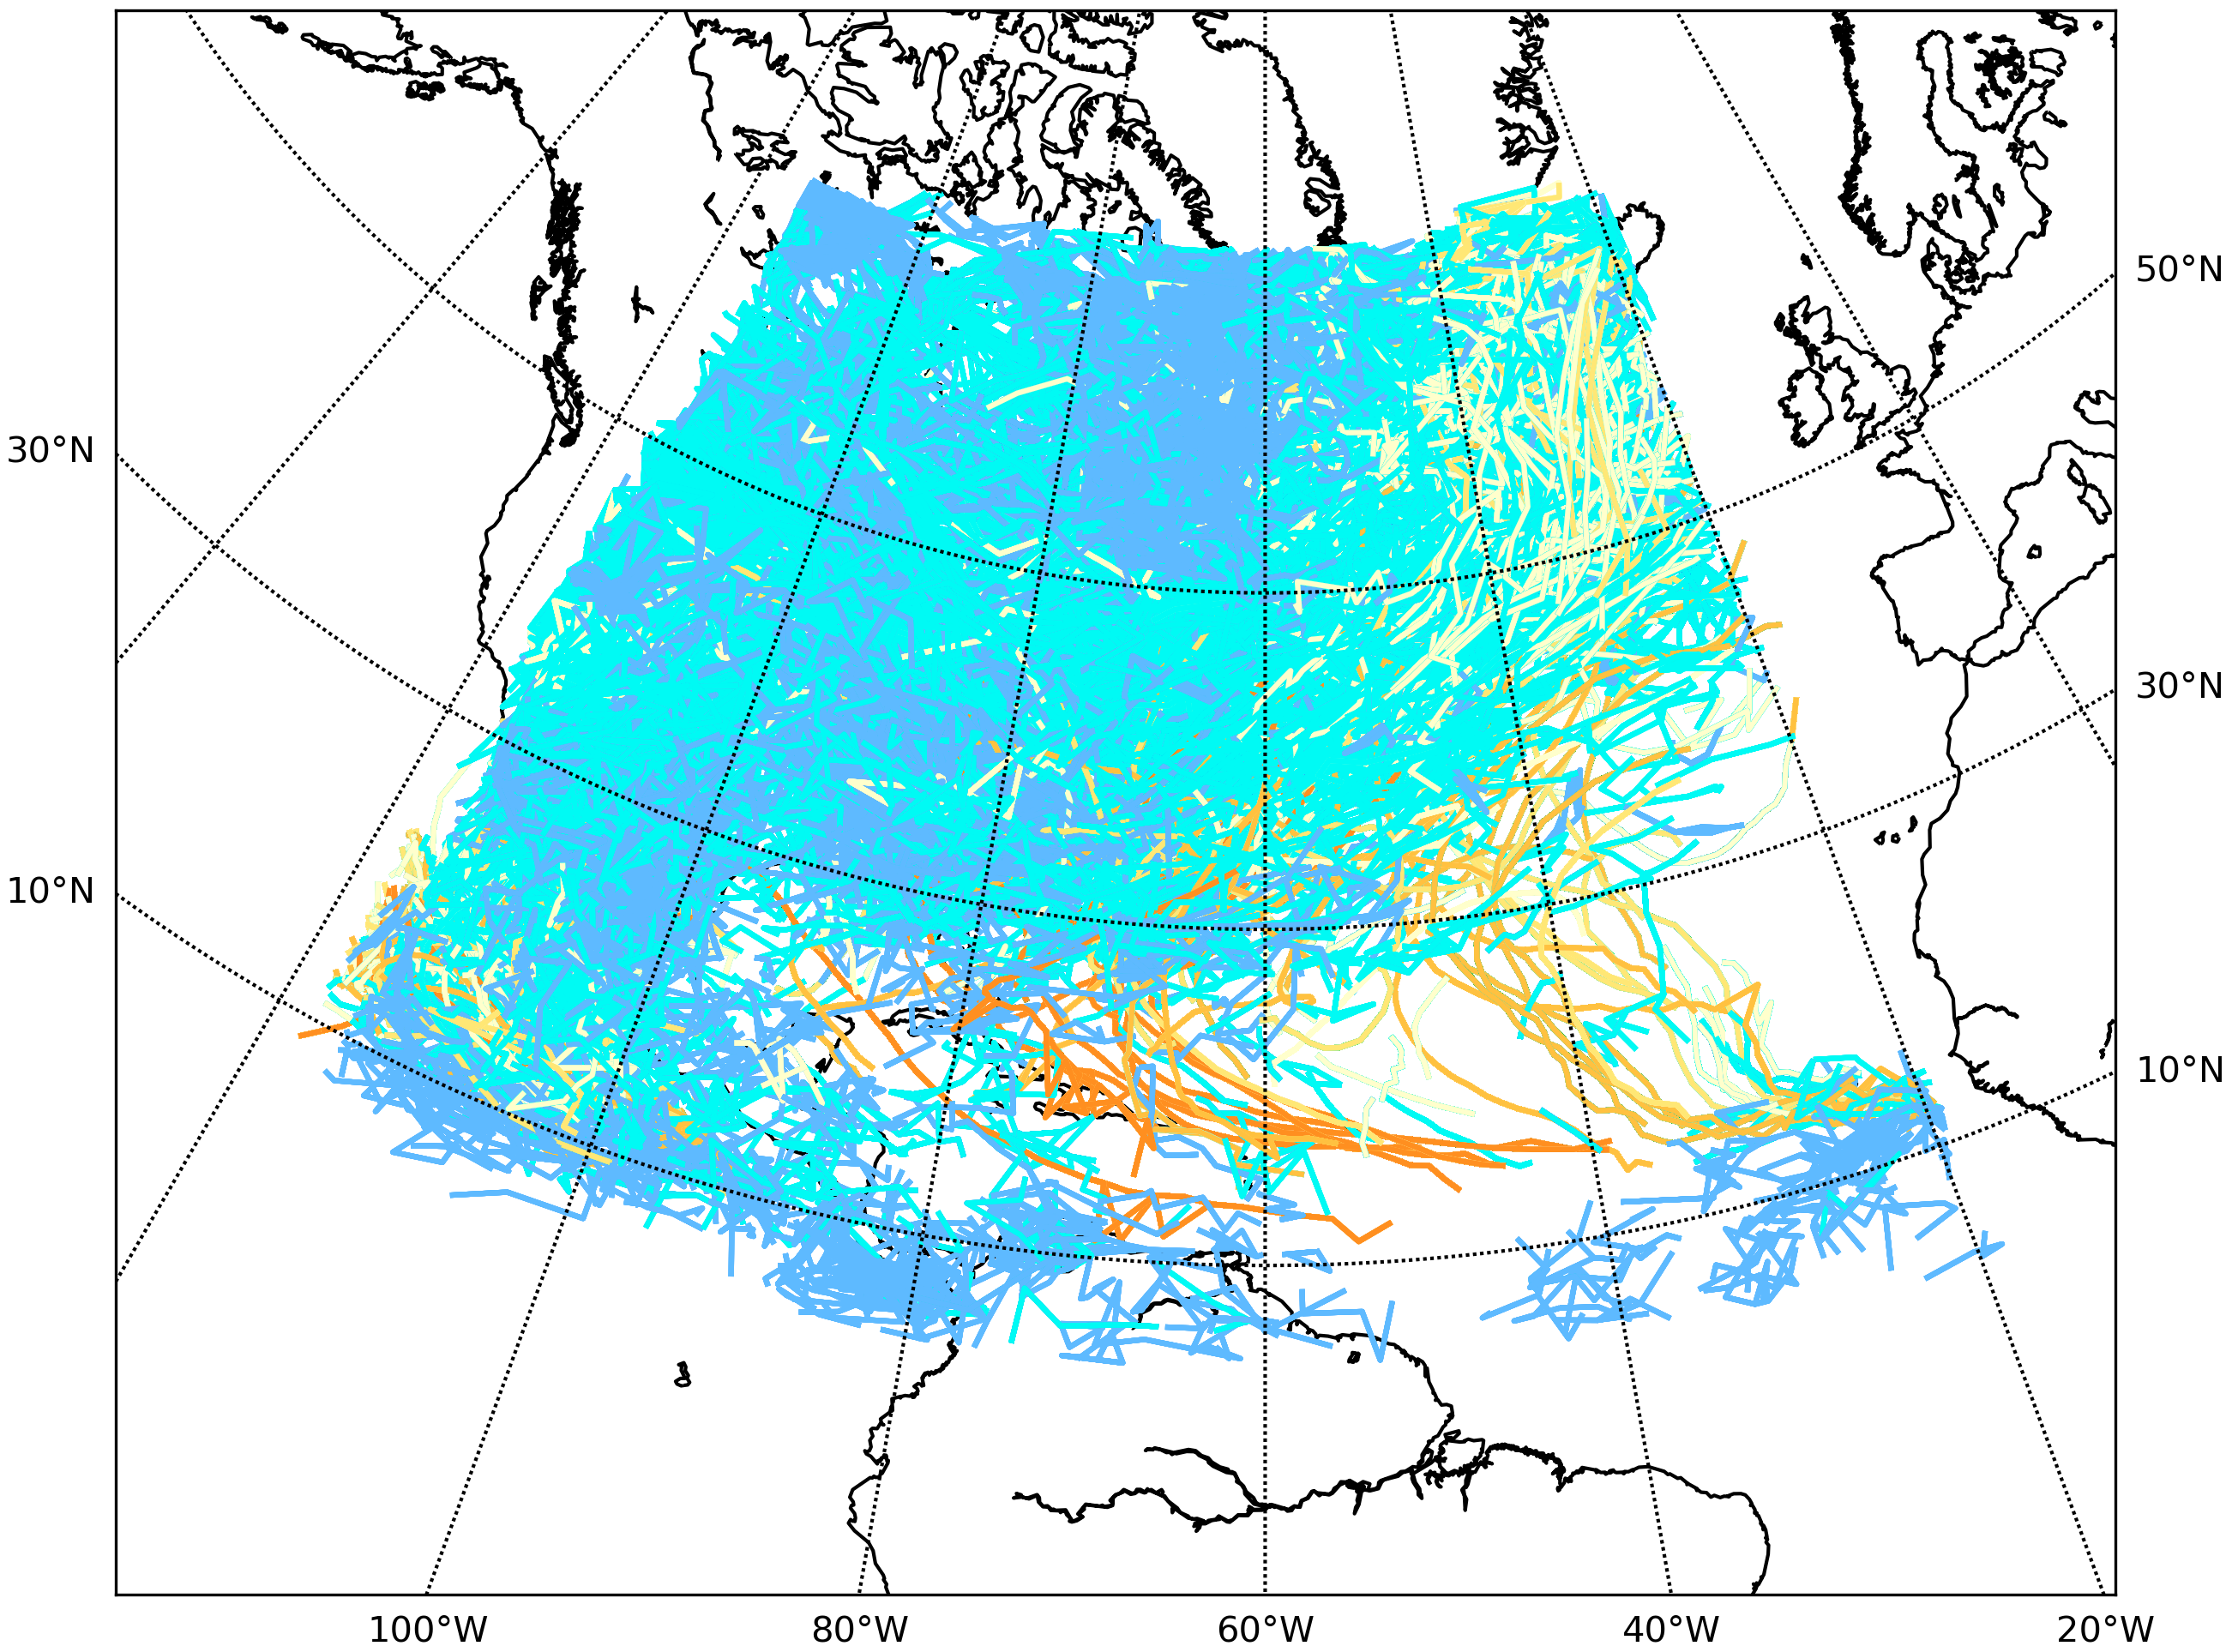
\includegraphics[width = \textwidth]{img/all_tracks.png}
	\end{minipage}
	\hfill
	\begin{minipage}[t]{0.48\textwidth}
		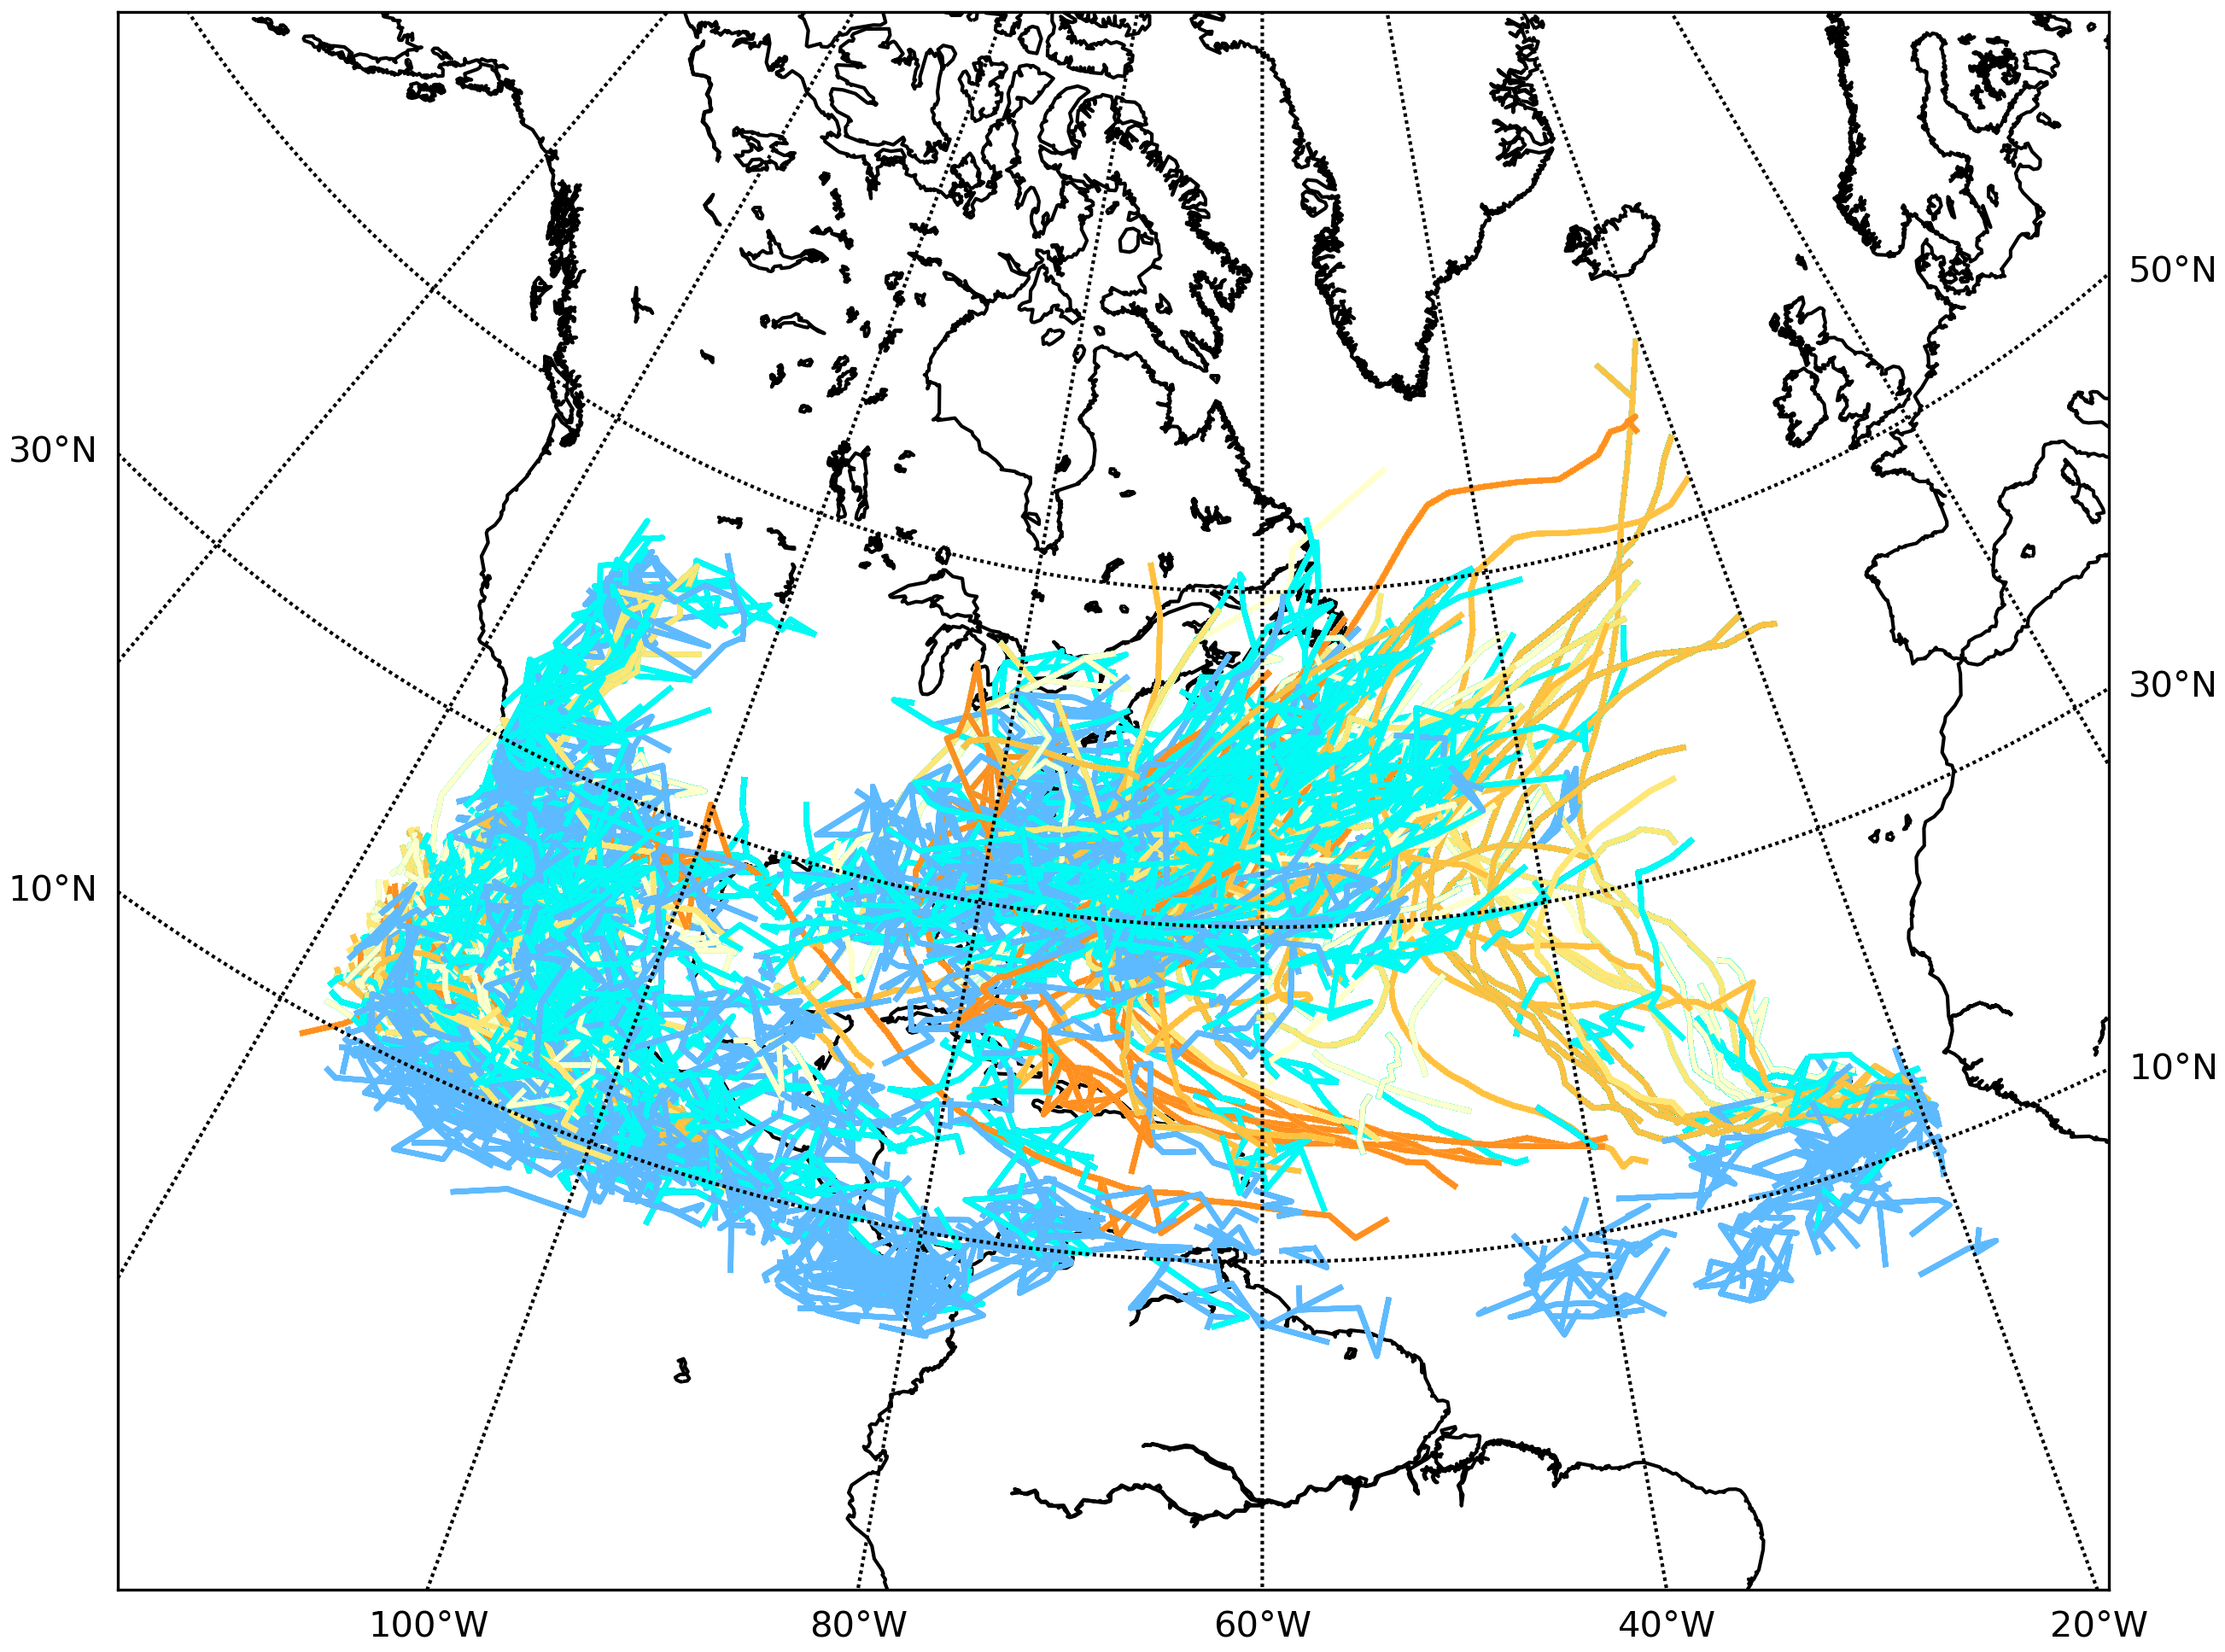
\includegraphics[width = \textwidth]{img/all_tracks_sst.png}
	\end{minipage}
	\caption{Comparison of all tracks without and with the SST criterion on the left and right}
	\label{fig:sst-effect}
\end{figure}
\subsection{Analysis of variation of parameters}
the following comparisons were performed